In this chapter we discuss the performance of our LSTM models. We discuss the implications 
our results and the results of similar works may have on the physical understanding 
of rainfall-runoff modelling. In addition we discuss potential ways to improve machine 
learning models for rainfall-runoff modelling, with focus on performance and 
interpretability.
\section{Model Selection}
\label{discuss model selection}
The results presented in Section \ref{CAMELS-GB results}-\ref{Mixed results} 
all agree that performance is increased when introducing static attributes. In 
addition to this, we see that the ordinary LSTM models that treat the static 
attributes as time series are the highest performing models. We find it likely that 
this is due  to the decrease in model complexity in an EA-LSTM compared to an LSTM. 
For example, Mixed$_\text{ea-lstm}$ has 205057 trainable parameters (weights and 
biases), Mixed$_\text{lstm}$ has 285953 and Mixed$_\text{none}$ has 266497. The 
EA-LSTM is a less complex model than an ordinary LSTM trained without 
static attributes. The EA-LSTM's performance coming close to that of an 
LSTM, while only using $~72\%$ of the trainable parameters is notable, however. 
It could imply 
that even a less complex model benefits from the additional information 
contained in the attributes. 
In all cases but the case of transfer learning, our best performing models are the 
most complex model with the highest amount of static attributes possible. For 
prediction on CAMELS-GB that means GB$_\text{lstm, all}$, for CAMELS the best model 
is US$_\text{Kratzert}$, for the datasets mixed the best model is Mixed$_\text{lstm}$, 
and for transfer learning: Transfer$_\text{US, none}$.

We do not spend significant time in this thesis tuning hyperparameters. Instead, 
we choose to use the hyperparameters derived by \citet{lstm_second_paper}. The one 
exception to this is for models trained on CAMELS-GB, shown in Section 
\ref{CAMELS-GB results}. We found 
that using dropout in this case at best makes no difference and at worst slightly 
decreases performance. In some cases we also tested whether increasing the 
sequence length from 270 days to 365 days increases performance, but our results 
indicate that this leads to no performance difference. To save memory and decrease 
training time we therefore keep the lower sequence length of 270 days.

We acknowledge that it may be possible to further increase the performance by doing 
a thorough hyperparameter tuning experiment. The tuning done by \citet{lstm_second_paper} 
is a simple grid search with few points, and is not guaranteed to be a good basis, 
especially since this tuning was done for gauged basin prediction. Hyperparameters 
are likely to have different optimal values for our case of ungauged prediction. A very thorough 
hyperparameter tuning would be hard to brute force, due to the computationally 
expensive nature of our models, therefore one would have to implement a more sophisticated 
method than mere exhaustive grid searching. This becomes even more computationally 
expensive if one wants to tune using cross validation.

We find no clear signs of overfitting in our selected models when comparing 
cross validated performance to test performance. Table 
\ref{results summary table} indicates 
similar performance between the cross validated models and the refit models 
validated on the test set. There are some discrepancies in the CDF plot of 
the performance of the models trained on CAMELS 
shown in Figure \ref{test cdf} (second from top), leading to a median NSE of 
0.65 on the test set as opposed to $0.68$ in the cross validated case. This small 
deviation could perhaps be explained by the findings of \citet{lstm_second_paper},
 which found that an ensemble of LSTM models performs better than a singular LSTM 
 because of nontrivial differences in performance caused by randomness in the 
 training process. For computational reasons we have chosen not to use model 
 ensembles anywhere in this thesis.

Aside from dropout in the final layer, we employ no regularization methods on 
our models. \citet{lstm_third_paper} 
argue that there is evidence that adding so-called "physical constraints" to 
models used on CAMELS could be helpful. This is argued because the LSTM models 
underperform compared to SAC-SMA on some basins. Here the paper compares SAC-SMA 
to an LSTM trained on all basins, training and validation split time series-wise 
and not basin-wise. SAC-SMA is a conceptual model and is therefore not usually seen 
as a purely "physical" model, but it is based more on physical arguments than a 
generalized machine learning method.
\begin{Huge}
    Remember to elaborate after writing theory
\end{Huge}
Still, both SAC-SMA and the LSTM are essentially 
parameter based models, without clear physical interpretations of most parameters. 
Because of this, we are unsure whether the argument that this is evidence for physical 
constraints is sufficient. More research is needed on the topic. Regularization in 
the form of physical constraints may yield several benefits, some of which could be
\citep{hybrid_paper}:
\begin{itemize}
\item Interpretability: Physical constraints could improve the physical interpretability 
of the LSTM.
\item Improved generalization: The goal of most machine learning regularization is 
to improve performance by increasing bias and decreasing variance (see Figure 
\ref{Bias Variance rainfall}). Increasing bias using physical laws would fit well 
into the narrative of \citet{BiasVarianceVIC} and \citet{VICbench}, although from 
the opposite angle. These papers argue that process-driven models are often too 
statistically constrained, due to them being driven almost entirely by interpretable 
physical processes. \citet{VICbench} showed that VIC performs at a higher level 
when tuning more parameters than usual, as these parameters are often pre-set based 
on physical a-priori knowledge. This is analogous to the bias-variance trade-off 
in machine learning. An LSTM is much less constrained and therefore performs better, 
agreeing with the results of the aforementioned papers. Making LSTM models 
slightly more constrained (as worded by \citet{BiasVarianceVIC}) could then make 
them generalize successfully to more basins while still being powerful enough to 
learn necessary relationships between input variables.
\end{itemize}
In the spirit of \citet{hybrid_paper}'s argument for increasing the physical consistency 
of models, we propose a simple semi-physical constraint:
\begin{equation}
\bm{\hat{y}} = \text{LSTM}(\bm{x}),
\end{equation}
where $\bm{\hat{y}}$ now consists of three outputs: $\bm{y}_\text{discharge}$, 
$\bm{y}_\text{frost}$ and $\bm{y}_\text{radiation}$. These represent runoff, 
frost/snow and radiated water respectively. Only $\bm{y}_\text{discharge}$ would 
be treated as the actual input when calculating the original cost function 
(\ref{NSE loss}). We then introduce a long term frost storage variable $\bm{W}^t_\text{frost}$.
For each time step this storage variable is updated by 
\begin{equation}
    \bm{W}_\text{frost}^{t+1} = \bm{W}_\text{frost}^t + \bm{y}_\text{frost},
\end{equation}
where $t$ is the current time step.
When calculating the loss function, we now add a new term to (\ref{NSE loss}):
\begin{equation}
    L = \text{NSE}^* + \gamma \left|(\bm{y_\text{discharge}} - \bm{x}_\text{precipitation} 
    - \bm{y}_\text{radiation} - (\bm{y}_\text{frost} - \bm{W}_\text{frost}))\right|
    \label{physical constraint}.
\end{equation}
Here $\gamma$ is a hyperparameter that needs to be tuned. Our reasoning 
behind (\ref{physical constraint}) is that this cost function penalizes models for 
making predictions where there is more runoff than available precipitation, 
snow and frost. Our hypothesis is that this penalty should lead to less complex 
models that are less likely to predict unphysical behaviors, leading to 
fewer NSE scores below zero. It could also improve interpretability of the model's 
output. Whether this or a similar constraint behaves as intended remains to be seen.

\begin{figure}
\centering


%\tikzset{every picture/.style={line width=0.75pt}} %set default line width to 0.75pt        

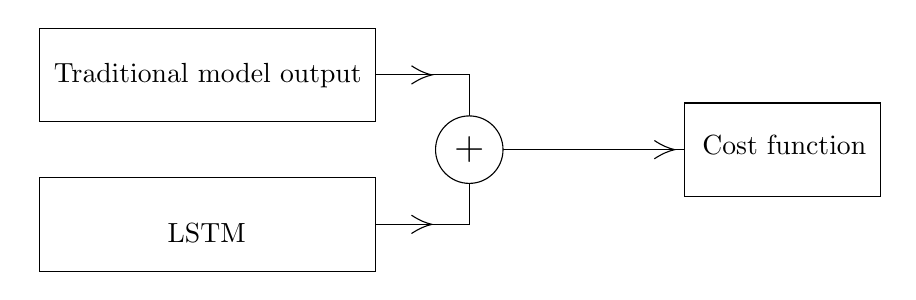
\begin{tikzpicture}[x=0.75pt,y=0.75pt,yscale=-0.9,xscale=0.9]
%uncomment if require: \path (0,300); %set diagram left start at 0, and has height of 300

%Shape: Right Angle [id:dp6736520719365272] 
\draw   (320,50) -- (370,50) -- (370,90) ;
%Shape: Right Angle [id:dp1824696211077277] 
\draw   (370,90) -- (370,130) -- (320,130) ;
%Straight Lines [id:da5169071611896188] 
\draw    (370,90) -- (485,90) ;
\draw [shift={(480,90)}, rotate = 180] [color={rgb, 255:red, 0; green, 0; blue, 0 }  ]   (10.93,-4.9) .. controls (6.95,-2.3) and (3.31,-0.67) .. (0,0) .. controls (3.31,0.67) and (6.95,2.3) .. (10.93,4.9)   ;
\draw [shift={(350,50)}, rotate = 180] [color={rgb, 255:red, 0; green, 0; blue, 0 }  ]   (10.93,-4.9) .. controls (6.95,-2.3) and (3.31,-0.67) .. (0,0) .. controls (3.31,0.67) and (6.95,2.3) .. (10.93,4.9)   ;
\draw [shift={(350,130)}, rotate = 180] [color={rgb, 255:red, 0; green, 0; blue, 0 }  ]   (10.93,-4.9) .. controls (6.95,-2.3) and (3.31,-0.67) .. (0,0) .. controls (3.31,0.67) and (6.95,2.3) .. (10.93,4.9)   ;
%\draw   (336,44.92) .. controls (340.03,47.37) and (344.07,48.84) .. (348.1,49.33) .. controls (344.07,49.82) and (340.03,51.3) .. (336,53.75) ;
%\draw   (338.5,130.08) .. controls (342.53,132.54) and (346.57,134.01) .. (350.6,134.5) .. controls (346.57,134.99) and (342.53,136.46) .. (338.5,138.92) ;

% Text Node
\draw    (140,25) -- (320,25) -- (320,75) -- (140,75) -- cycle  ;
\draw (230,50.2) node   [align=left] {\begin{minipage}[lt]{122.67200000000003pt}\setlength\topsep{0pt}
\begin{center}
Traditional model output
\end{center}

\end{minipage}};
% Text Node
\draw    (140,105) -- (320,105) -- (320,155) -- (140,155) -- cycle  ;
\draw (229.4,134.6) node   [align=left] {\begin{minipage}[lt]{122.67200000000003pt}\setlength\topsep{0pt}
\begin{center}
LSTM
\end{center}

\end{minipage}};
% Text Node
\draw  [fill={rgb, 255:red, 255; green, 255; blue, 255 }  ,fill opacity=1 ]  (370, 90) circle [x radius= 18.06, y radius= 18.06]   ;
\draw (370,90) node   [align=left] {\begin{minipage}[lt]{16.864pt}\setlength\topsep{0pt}
\begin{center}
{\Large +}
\end{center}

\end{minipage}};
% Text Node
\draw    (485,65) -- (590,65) -- (590,115) -- (485,115) -- cycle  ;
\draw (538.6,87.4) node   [align=left] {\begin{minipage}[lt]{68pt}\setlength\topsep{0pt}
\begin{center}
Cost function
\end{center}

\end{minipage}};


\end{tikzpicture}

.tex}
    \caption[Potential simple hybrid model.]{Sketch of how a simple hybrid model could be implemented. The traditional model and the LSTM model are completely separate, making it unnecessary to calculate gradients for the traditional model. The idea here would be for the LSTM model to learn the phenomena lacking in traditional models.}
\label{figure simple hybrid}
\end{figure}
Sticking to the topic of increased generalizability and interpretability, we 
believe it to be of interest to implement a hybrid model, i. e. a machine learning 
model implemented alongside or as part of a 
traditional model. The machine learning model either replaces parts of or supplements 
the predictions of a traditional model. A very simple implementation of this is shown 
in Figure \ref{figure simple hybrid}. This model would take the same inputs as 
the models trained in this thesis, but the cost function would be calculated on 
the sum of the output of the traditional model and the machine learning model. 
This means that the machine learning model learns to correct 
the errors of a given traditional model instead of doing actual prediction.

This thesis and earlier research done by \citet{lstm_first_paper,lstm_second_paper,lstm_third_paper} 
are all limited to simple LSTM models. LSTM models are, due to their recurrent nature, 
notoriously slow. Graphics cards and similar highly parallel computational devices 
are not optimized for recurrent calculation. A relatively 
simple way to surpass this could be to implement a one-dimensional 
Convolutional Neural Network (CNN) layer as the first layer of our model. This 
layer could then be used to reduce the time resolution of the data, still retaining 
information. The usage of CNNs for time series prediction is becoming increasingly
widespread \citep{CNN-timeseries}. We still argue that LSTM models fit the type of
physical system modelled in this thesis very well and is logically consistent 
with the way rainfall-runoff 
models are typically structured, but using a CNN layer to improve performance 
should not detract from this.

\section{Performance and Importance Analysis}
\label{discuss static attributes}
\subsection{CAMELS-GB}
Table \ref{overfit table} shows among others \textbf{\texttt{Q95}} as the most 
important attribute for the overfit "proof of concept" model. This attribute is the 
95th percentile runoff value for the full runoff time series for a given basin, 
which is information directly derived from the expected outcome. 
Figure \ref{CAMELS-GB CDF validation} also shows that the overfit model drastically 
outperforms all other models.
Because of this, we believe it is 
safe to assume that an LSTM model can learn which static attributes are 
the most important in CAMELS-GB, at least in the most obvious case. In addition, 
it also indicated that the permutation test succeeds at deciding the most important 
static attribute in this case. These assumptions are therefore used to strengthen 
our confidence in the results from our other, non-overfit models. 

Looking again at Figure \ref{CAMELS-GB CDF validation} along with Table 
\ref{results summary table}, we see that the median NSE value of GB$_\text{lstm, all}$ 
is approximately $0.82$ cross validated, with a test score of $0.80$. 
This performance is vastly superior to that found by \citet{lstm_third_paper}, and 
is even better than gauged prediction on CAMELS, such as \citet{lstm_second_paper}. 
This makes sense when one considers the relatively low variance in climate in Great 
Britain, compared to the United States. 
As far as the author knows, there are no published benchmarks using traditional models on 
CAMELS-GB. Creating such a benchmark in the future is necessary for us to properly 
assess model performance.

In Figure \ref{best prediction all concat seq len}, we see that at least for the 
best performing prediction, the high NSE score does 
in fact transfer to a visually impressive performance. Despite some peaks not being 
correctly simulated, the LSTM model manages to replicate the observed runoff in a 
very acceptable manner.

As the results presented in Table \ref{all concat table}
indicate that the many of the important static attributes in CAMELS-GB (as perceived by 
GB$_\text{lstm, all}$) are derived directly from the 
input time series, it is likely that we cannot extract much new information from 
these, as this information should be available in the time series already used by 
the models. The reason for this is being the case is likely connected to the 
nature of the LSTM training process and the sequence length. Ways 
to further improve the long-term memory of an LSTM should be further explored 
in the future. The biggest examples of this type of attribute are the top two ranked 
attributes: \textbf{\texttt{low\_prec\_dur}} and \textbf{\texttt{low\_prec\_freq}}. 
These severely outrank all other static attributes, especially for the 75th percentile 
of importances, and they are directly derived from the precipitation time series.
Other than derived features, the model ranks the other attributes relatively similarly 
for the upper 75th percentile. These other attributes mostly contain information 
about land cover and elevation levels, which is information an LSTM cannot access 
through the time series contained in CAMELS-GB. Process-driven models such as VIC 
use information such as land coverage and elevation by splitting the catchment 
into a spatial grid, it is therefore unlikely that any of these attributes can 
contribute to any major improvements for process-driven models for predicting 
on CAMELS-GB. To summarize: Our model tends to mostly prefer static attributes 
containing information already available in the time series, it is therefore hard 
to argue that the static attribute ranking found here can be used to improve 
traditional models, which already use this information via the time series.

\subsection{CAMELS}
Looking at Figure \ref{CAMELS-US CDF validation} and Table \ref{results summary table}, 
the performance of US$_\text{Kratzert}$ coincides with the results of \citet{lstm_third_paper}, 
which is what we wanted to replicate. The performance is generally lower than that 
of GB$_\text{lstm, all}$, which makes sense when one considers how much more diverse 
the United States climate is, compared to the climate of Great Britain. 

The best prediction made by US$_\text{Kratzert}$ is very accurate and has an NSE of $0.92$. 
This is lower than for the best prediction on CAMELS-GB. Similarly to the previous 
section, we here too
see that the prediction fails to predict the higher peaks of runoff. 
This is also something observed by \citet{lstm_first_paper}.

Table \ref{kratzert importance} shows that the permutation test yields different 
results than the feature ranking done by \citet{lstm_second_paper}. Said paper 
averaged the normalized sensitivity (derived by what they call the explicit Morris 
method) of each basin, while we present percentiles and rank based on the median
\footnote{Also note that we predict on ungauged basins, in contrast to said paper. 
This could differentiate important attributes.}. 
Looking our median scores, we see that the majority of basins do not benefit 
from the inclusion of static attributes. Looking at the upper percentiles, the 
most important attributes in our case still somewhat agree with those of 
\citet{lstm_second_paper}. Topological information and climatic indices are important. 
By far the most important attributes for the 75th percentile are aridity and 
catchment area. Our results do however favour land coverage types and soil types 
more than the results of \citet{lstm_second_paper}, and the attribute deemed the most important by 
said paper, \textbf{\texttt{p\_mean}}, is only significantly important 
for the 95th percentile of basins. As expected, \textbf{\texttt{frac\_snow}} is 
much more important for CAMELS than for CAMELS-GB, as there is more snow 
in certain regions in the United States than in Great Britain. This is also reflected in the fact that 
\textbf{\texttt{frac\_snow}} is important for a small portion of British basins (the 95th percentile), 
while it is more important both for the 75th and 95th percentile in the US. 

\subsection{Mixed model}
Our best model trained on both CAMELS and CAMELS-GB seems to find static attributes
more important 
than the models trained on the datasets individually. Table \ref{importance mixed} 
shows that the model also ranks the attributes differently. Figure \ref{mixed CDF validation} 
shows that the addition of static attributes is of significantly higher benefit for 
prediction on CAMELS-GB than for CAMELS although the performance per dataset is not 
very far off the individually trained models (see Figure \ref{results summary table}).
This could be consistent with the importance rankings, as 
the median importances, and especially the 75th percentile and above importances, are 
significantly higher on CAMELS-GB than those on CAMELS. There is a chance that this 
is due to the model learning to use the attributes to differentiate between the 
two datasets, without actually extracting important information.

An interesting detail is that the permutation test yields negative importance 
for some basins. This happens for all models mentioned in this section. 
This implies that our LSTM models actually perform worse 
on some basins because of the inclusion of static attributes, perhaps due to a 
lack of training data representing similar basins in the dataset. This is likely 
alleviated by introducing more data. We believe other ways to rank attributes 
should also be attempted 
in the future. \citet{lstm_second_paper} used a robustness test which 
involves gradually adding Gaussian noise to a feature and checking how much it 
affects model performance (DOUBLE CHECK THIS!!!). \citet{OrigCAMELSRanking} 
uses a different method altogether, the results of which \cite{lstm_second_paper} 
agree with. To our knowledge there exists no feature ranking results on CAMELS-GB 
apart from what is shown in this thesis, 
so these two other methods should also be attempted on CAMELS-GB in addition 
to the permutation test employed in this thesis to get further context and comparability.

\subsection{Transfer learning}
The results in Section \ref{Transfer learning section} show that the models trained 
for transfer learning do not benefit from adding static attributes. Therefore, we 
do not include a permutation test for this case, We also see 
that the case of US$\rightarrow$GB significantly improves when removing attributes. This makes 
sense as Great Britain has much smaller climatic variance than the United States 
(see for instance Figure \ref{attribute comparison}). We believe these two phenomena could be related. It is likely 
that the relatively lower performance from using static attributes comes from the 
fact that the datasets have different climatic conditions. There could also be 
room for improvement in how we preprocess both the attributes and the time series. 
As seen in Table \ref{attribute transfer} we assume that the temperature time series 
of CAMELS behave like symmetrical periodic functions, therefore leading to 
\begin{equation}
T_\text{average} \approx  \frac{T_\text{min}+T_\text{max}}{2}. \label{dumb assumption}
\end{equation}
Ideally, we need to have temperature as a time series for a given model to be able 
to properly model snow and frozen soil accumulation, which is very important for 
hydrologic models. The fact that models trained on both datasets 
still perform comparably to models trained on only one dataset seems to suggest 
that (\ref{dumb assumption}) is not entirely destructive, however.
In the later stages of this thesis it was discovered that the average temperature 
is actually present in CAMELS. The older forcing data \citep{maurer} contains 
this information stored as duplicates in the maximum and minimum temperature time 
series. Due to time constraints, we are unable to train models utilizing this. 
This is likely a good start for those looking to improve transfer learning performance. 
The best outcome is likely to come from finding maximum and minimum temperatures 
for CAMELS-GB, however.

It seems to us that there are several angles to further tackle the issue of transfer 
learning between these datasets. One of which we stated above: Find maximum and minimum time series for 
CAMELS-GB. A second way is to improve the preprocessing of static attributes to 
the point where one would hopefully see better performance with attributes than 
without. 

While we state earlier in this chapter that we see no clear signs of overfitting, this is not 
the case for transfer learning. Figure 
\ref{training progress transfer} indicates that Transfer$_\text{GB, none}$ 
and Transfer$_\text{US, none}$ start overfitting on their respective training 
datasets at epoch one and five respectively. This overfitting is not apparent when
validating on basins from the 
same dataset as they are trained on, but very quickly manifests when validating 
on the other dataset. While improved pre-processing, regularization and the gathering 
of more  cross-compatible data could alleviate this problem, it is likely that this 
overfitting is 
unavoidable using the current datasets. More data, both in quantity and in 
diversity, is likely needed for the model's training process to be able to 
successfully predict on a dataset not included during training.

There now exist several other similar datasets to the two used for this study. 
The easiest way to improve 
any machine learning model is often to provide more data for training. A Chilean 
dataset consisting of 515 catchments by the name CAMELS-CL \citep{CAMELS_CL} 
was studied early in this thesis work, but the quality 
of the data was deemed worse than that of CAMELS and CAMELS-GB. With some initial 
preprocessing it could be of interest to see whether it is feasible to use this 
dataset.
In addition we know of two other datasets. One goes by the name CAMELS-BR, and is 
a Brazilian dataset consisting of 897 catchments \citep{CAMELS_BR}.
The other is CAMELS-AU, and is an Australian dataset consisting of 222 catchments
 \citep{CAMELS_AU}. Especially CAMELS-BR seems to be of interest due to the 
amount of catchments. Combining datasets is a non-trivial, time consuming task, which 
we expect will become increasingly hard the more datasets one tries to combine. 
It is not unlikely that one has to discard almost all static attributes to make 
the datasets compatible. We therefore expect that some effort to gather new data 
would also be necessary. It is of course also of interest to see how well machine 
learning models perform on one or more of these datasets in isolation. 
We see this as a possible candidate for the start of a new master thesis.
\section{Comparison to traditional models}
We are able to reproduce the results of \citet{lstm_second_paper,lstm_third_paper}. 
Our models 
trained on CAMELS perform significantly better than traditional models. In this 
thesis we compare to two process-driven models, VIC and NWM, and one conceptual 
model, SAC-SMA. 

What we additionally show in this thesis is that models trained on both CAMELS and CAMELS-GB 
also perform better on CAMELS than the addressed traditional models. This could 
be because the models are complex enough to recognize which dataset a given 
basin is from based on underlying signatures in either the time series or the 
static attributes. Perhaps this differentiation could stem from differences in 
data collection practice. 

One of many reasons why LSTM models perform better than traditional models on CAMELS in general 
could be that the LSTM 
models are better at modelling basins with special conditions leading to 
a rainfall-runoff ratio different from 1. When the rainfall-runoff ratio is lower 
than one it usually implies that the rainfall is either stored as snow or frozen 
soil, that it is vaporized through photosynthesis in local vegetation, or that there 
is some difficult to model complexity to the subsurface flow in the area. 
These processes are difficult to model compared to runoff directly caused by 
rainfall \citep{process-driven-history}.
Our results may indicate that this could be the case.
Figure \ref{runoff ratio} shows that only the traditional models have 
a statistically significant linear relationship between performance and 
rainfall-runoff ratio. The relationships are generally weak, with a Pearson 
correlation between 0.24 and 0.33, but they are more apparent than 
for the LSTM models, where there exists no such linear relationship. The impact 
of this discovery is quite uncertain, however, as there is significant 
Spearman correlation (nonlinear correlation) for all the models, ranging 
from 0.31 to 0.53.

The LSTM models are, as briefly mentioned earlier, much less complex spatially. 
While process-driven models (check SAC-SMA as well though idiot!) need to grid the 
spatial dimension to properly model the physical system, an LSTM model finds 
relationships between input and output data in a one-dimensional manner. This could 
make LSTMs and other machine learning methods valuable models to use when there is not 
enough data available to properly set up a traditional model such as the NWM.
